\documentclass[a4paper,11pt]{article}
\usepackage[margin=2cm]{geometry}

\usepackage[toc,page]{appendix}
\usepackage[nodayofweek]{datetime}
\usepackage{cite}
\usepackage{graphicx}
\longdate

\usepackage{hyperref}
\usepackage{fancyhdr}
\pagestyle{fancyplain}
\fancyhf{}
\lhead{\fancyplain{}{M.Sc.\ Group Project Report}}
\rhead{\fancyplain{}{\today}}
\cfoot{\fancyplain{}{\thepage}}


\title{Implementation of attentional bistability of the dragonfly visual neurons in an intelligent biomimetic agent\\\Large{--- Report Two ---}}
\author{Juan Carlos Farah, Panagiotis Almpouras, Ioannis Kasidakis, Erik Grabljevec, Christos Kaplanis\\
       \{jcf214, pa512, ik311, eg1114, ck2714\}@doc.ic.ac.uk\\ \\
       \small{Supervisors: Professor Murray Shanahan, Zafeirios Fountas, Pedro Mediano}\\
       \small{Course: CO530/533, Imperial College London}
}

\begin{document}
\maketitle
\section{Challenges and Motivation for New Specification}
In this section, we motivate our change in specification by highlighting the biggest challenges that we have encountered in our project. 

Our most significant challenge has been to generate the output we expect from the CSTMD1 neurons, given an input from the initial visual processing (the ESTMDs). In part (iii) of Stage 1A as specified in Report 1, we expected to observe evidence that the CSTMD1 selects one target between two that are presented in the visual receptive field. The CSTMD1 model is not currently displaying this selectivity as shown in Figure 1. What we expected was that the firing rate graph for both targets would emulate that of one of the two targets, but instead it usually just fire more when both targets are presented. 
	\begin{figure}[h]
	\begin{center}
	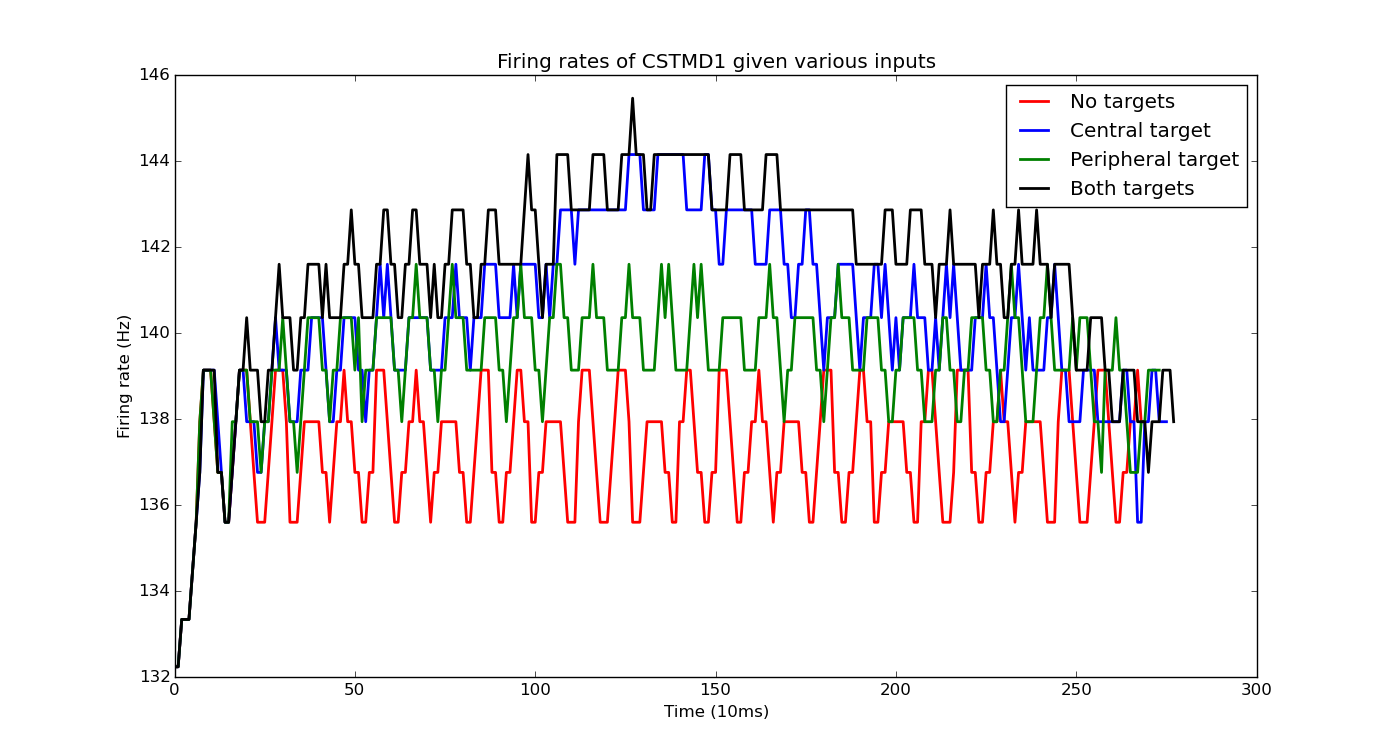
\includegraphics[scale = 0.3]{firingrates}
	\end{center}
	\caption{Firing rates of CSTMD1}
	\end{figure}	

Given the complicate nature of the morphologically modelled CSTMD1 (which is largely third party code) and the fact that this target selection has never been shown before in a CSTMD1 model, we are concerned that we may not be able to reproduce this phenomenon shown by biological CSTMD1 neurons within the time constraints of this project. While it is still our goal to do so, we are moving this part of the specification out of minimum requirements and into possible extensions.
In light of this, we thought that what might be useful instead is to create a webtool that enables the user to:
\begin{enumerate}
	\item Modify key parameters in each of the components of our dragonfly visual system.
	\item Run each component individually and display key metrics demonstrating the functionality of each component.
	\item Run the components in unison and display key metrics demonstrating the functionality of the system as a whole.
\end{enumerate}
This would enable us, or an external user, to efficiently investigate the properties of our dragonfly visual system and better tune the parameters in order to achieve target selection and prey capture in our model.

\section{New Specification}
Below we layout our new requirements and the stage of completion for each part:
\begin{center}
    \begin{tabular}{p{12cm} c c}
    \textbf{Minimum Requirements (Stage 1)} & \textbf{Completion} \\ \hline
    (A)(i) Create an animation tool to create inputs for the visual processing & Full \\ 
	(A)(ii) Build a model of the visual processing (ESTMD) that occurs between the retina and the actual CSTMD1 neurons of a real dragonfly & Full \\
	(A)(iii) Decide how many CSTMD1 neurons we will use and how exactly to connect them to the output of our visual processing & Full \\
	(B) Build a layer of pattern recognition neurons that can learn to recognise spike patterns within a noisy input & Full\\
	(C) Integrate the visual processing and pattern recognition system to detect patterns within the CSTMD output and add a simple action-selection mechanism. & Partial\\
    \end{tabular}
\end{center}

\begin{center}
    \begin{tabular}{p{12cm} c c}
    \textbf{Expected Implementation (Stage 2)} & \textbf{Completion} \\ \hline
	(A) Develop webtool to analyse metrics of each component of the dragonfly visual system & Partial \\
	(B) Create a virtual 3D environment for the dragonfly agent & None\\
	(C) Enhance the action selection mechanism to control the agent within the environment & None\\
    \end{tabular}
\end{center}

\begin{center}
    \begin{tabular}{p{12cm} c c}
    \textbf{Possible Extensions (Stage 3)} & \textbf{Completion} \\ \hline
	(A) Succeed in getting the CSTMD1 to exhibit target selection by changing parameters and the connection with the ESTMD & Partial\\
	(B) Improve usability and features of webtool. & None\\
	(C) Implement the agent in a quadcopter drone & None\\
    \end{tabular}
\end{center}


\section{Progress}

\begin{enumerate}

	\item Animation tool. The animation tool, created using Pyglet, gives the user the option to create a video of black targets moving across a custom background that is either stationary or moving. The size and velocity vector of each target is adjustable.
	\item Visual processing. We successfully implemented a model for ESTMD (elementary small-target-motion detectors) based on \cite{hal11}. The model can detect small-target motion across a moving, complicated background. This stage required a lot of research and understanding of spatio-temporal filters that approximate the function of real ESTMD neurons. The input of the ESTMD can either be a full video or frame by frame as it is produced by the animation tool. The output of the ESTMD model is a time series of matrices of processed pixels, which can be viewed in a video. See screenshots of videos in Appendix A.
This output is connected to the CSTMD neurons by converting each pixel into a firing rate for a simple integrate-and-fire neuron and connecting the output of each of these neurons to the CSTMDs, biasing the weights of the centre of the visual input with a Gaussian distribution.
	\item Pattern recognition. To model the pattern-recognition neurons needed for our project, we initially replicated experiments conducted by T. Masquelier et al. (Citation Needed). The resulting code was a Python module for Spike Response Model (SRM) Leaky Integrate-and-Fire (LIF) neurons that successfully recognised input patterns based on the samples described in the respective papers. A single of these neurons is able to successfully recognise a recurring pattern within background noise and a network of them is able to do so for multiple patterns. We then extended the module so that the neurons can be easily adapted to recognise input with varying properties such as average firing rate, number of afferents, frequency with which the pattern appears, amongst others. This implementation is able to recognise patterns output from our CSTMD1 neurons and measures the effectiveness of the pattern-recognition neurons by tracking key information such as true-positive, false-positive and true negative spike incidences.
\end{enumerate}

\section{Updated Task Scheduling}	

Below is a condensed version of our updated schedule.

\subsection{Stage 1C: Connecting CSTMD to pattern recognition}
\begin{center}
    \begin{tabular}{p{12cm} c c}
    \textbf{Task} & \textbf{Priority} & \textbf{Sprint} \\ \hline
	Get pattern recognition to recognize small patterns from CSTMD output & 1 & 3/4 \\
	Get second layer of pattern recognition neurons to recognize longer patterns & 1 & 3/4\\
	Create simple action selection mechanism. & 1 & 4 \\
    \end{tabular}
\end{center}

\subsection{Stage 2: Webtool and Enhanced Action selection}
\begin{center}
    \begin{tabular}{p{12cm} c c}
    \textbf{Task} & \textbf{Priority} & \textbf{Sprint} \\ \hline
    Define range of actions available to biomimetic agent & 2 & 4 \\
    Design and implement basic environment for simulated agent & 2 & 4/5 \\
    Implement adapted Braitenberg vehicle as action selection mechanism & 2 & 4/5 \\
	Parametrize components of visual system for integration into webtool & 2 & 4 \\
	Integrate classes of components into webtool & 2 & 4/5 \\	
	Implement useful metrics for each component in webtool & 2 & 4/5 \\
    \end{tabular}
\end{center}

\subsection{Stage 3: Target selection and improve webtool}
\begin{center}
    \begin{tabular}{p{12cm} c c}
    \textbf{Task} & \textbf{Priority} & \textbf{Sprint} \\ \hline
    Get CSTMD to select between targets & 3 & 3-6 \\
    Implement agent in a quad-copter drone & 4 & 6/7 \\
    \end{tabular}
\end{center}

\section{Testing Methodology}

\section{Testing results}

\bibliography{report2}{}
\bibliographystyle{plain}

\begin{appendices}
\section{Animation / ESTMD screenshots}
\section{Testing results}

\end{appendices}

\end{document}

